
\subsubsection{The Merchant Edge}

The merchant edge is the link between two merchants when a single client have transacted at both as depicted in fig \ref{fig:graphexample}.  This merchant-merchant relationship, here called TRIADIC\_MERCHANT\_FEET\_LINK, see fig \ref{fig:triadic_closure}, is said to close the triangle between client and two merchants. 
Clients make a choice to visit and transact at more than one merchant. The period under consideration may be extended to include all history for a client in which case the preference and geographical insight will presumably be much weaker.  At the other extreme the period may be restricted to a particular day.  In such an event, triadic closure is only achieved when a transaction is concluded at two merchants on the same day.  

\begin{figure}[htb!]
\caption{Triadic closure between merchants}
\centering
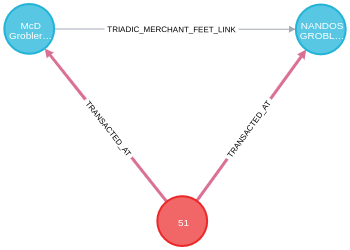
\includegraphics[width=\textwidth]{triadic_closure.png}
\label{fig:triadic_closure}
\end{figure}

TRIADIC\_MERCHANT\_FEET\_LINK has three properties.  All three properties are the result of a transaction count, as opposed to transaction value, and hence the reference to feet.  Given a merchant A and a merchant B, the first is \textbf{count}, which is the number of clients who transacted at both merchants A and B, count also provides a means of attaching a weight to TRIADIC\_MERCHANT\_FEET\_LINK and a convenient means of eliminating weak and spurious relationships.
The second property is a count of all transactions performed at A by clients who transacted at A and B, ID0.  The third property is similarly the count of all transactions performed at B by clients who transacted at A and B, ID1.  ID0 and ID1 provides a means of establishing a direction for the merchant feet edge: if ID0\<ID1, then the merchant edge points in the direction of B and in the direction of A if ID1\<ID0.  The direction property of TRIADIC\_MERCHANT\_FEET\_LINK becomes important when ranking merchants.
These three properties provide the strength of the edge between A and B but also a means to attach a direction to the edge by pointing it in the direction of the net count of transactions.
Triadic closure creates a relationship between two merchants that were not immediately apparent from the data.

\paragraph{The value edge}

The value edge also establishes a direction of a merchant edge.  Using a transaction value for each of the linked merchants, but only for clients who shopped at merchant A and also B, if the total value of all transactions for this client at B is larger than at A the 'value' for this client is flows from A to B for this client.  When aggregated over the period for all clients an aggregated 'value' direction is established.
